\documentclass[tikz,border=14pt]{standalone}
\usepackage{tikz}
\usepackage{amsmath}
\usepackage{amssymb}
\usetikzlibrary{arrows.meta,calc}

%% ── colour palette ────────────────────────────────────────────────────────
\definecolor{cE} {RGB}{189,214,232}   % embed   – steel blue
\definecolor{cH} {RGB}{213,190,232}   % Hopfield – lavender
\definecolor{cGa}{RGB}{255,213,153}   % gate     – amber
\definecolor{cGr}{RGB}{187,228,187}   % graph    – sage
\definecolor{cP} {RGB}{248,198,192}   % predict  – rose
\definecolor{cBk}{RGB}{226,218,243}   % bank     – soft purple
\definecolor{cOr}{RGB}{155, 68,  4}   % gate title text – dark orange

\begin{document}
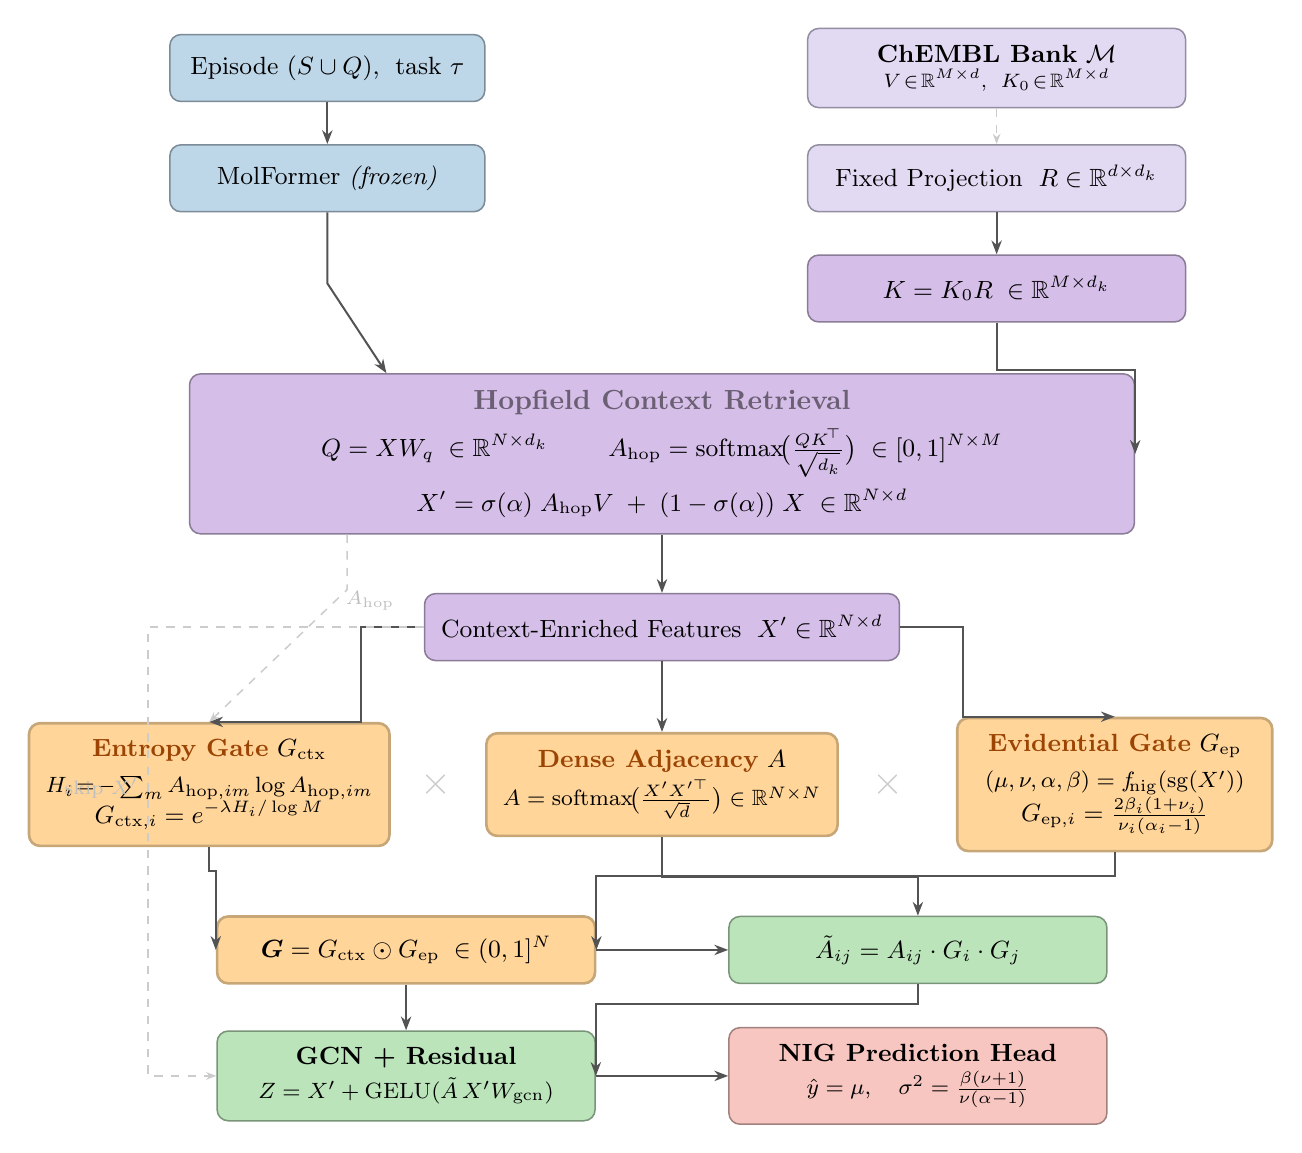
\begin{tikzpicture}[font=\small,
  arr/.style ={-{Stealth[scale=0.80]}, line width=0.72pt, gray!65!black},
  darr/.style={-{Stealth[scale=0.68]}, line width=0.55pt, gray!40, dashed},
  E/.style ={rectangle, rounded corners=4pt, text centered, inner sep=6pt,
             minimum height=0.85cm, line width=0.55pt,
             draw=cE!65!black, fill=cE},
  H/.style ={rectangle, rounded corners=4pt, text centered, inner sep=6pt,
             minimum height=0.85cm, line width=0.55pt,
             draw=cH!65!black, fill=cH},
  Ga/.style={rectangle, rounded corners=4pt, text centered, inner sep=6pt,
             minimum height=0.85cm, line width=0.95pt,
             draw=cGa!78!black, fill=cGa},
  Gr/.style={rectangle, rounded corners=4pt, text centered, inner sep=6pt,
             minimum height=0.85cm, line width=0.55pt,
             draw=cGr!65!black, fill=cGr},
  P/.style ={rectangle, rounded corners=4pt, text centered, inner sep=6pt,
             minimum height=0.85cm, line width=0.55pt,
             draw=cP!65!black, fill=cP},
  Bk/.style={rectangle, rounded corners=4pt, text centered, inner sep=6pt,
             minimum height=0.85cm, line width=0.55pt,
             draw=cBk!65!black, fill=cBk},
]

%% ── x positions ───────────────────────────────────────────────────────────
\def\xEp{3.50}    % episode / MolFormer
\def\xBk{12.00}   % ChEMBL bank / fixed R / projected keys
\def\xHc{7.75}    % Hopfield centre (wide block)

\def\xGL{2.00}    % Entropy Gate centre
\def\xGC{7.75}    % Dense Adjacency centre
\def\xGR{13.50}   % Evidential Gate centre

\def\xBL{4.50}    % Combined G / GCN
\def\xBR{11.00}   % Gated à / NIG

%% ── y positions ───────────────────────────────────────────────────────────
\def\yRA{ 0.00}   % episode + bank
\def\yRB{-1.40}   % MolFormer + fixed R
\def\yRC{-2.80}   % projected keys
\def\yHp{-4.90}   % Hopfield wide block (tall, 3-line)
\def\yXP{-7.10}   % X' enriched
\def\yGt{-9.10}   % gate row
\def\yCG{-11.20}  % combined G + gated Ã
\def\yGN{-12.80}  % GCN + NIG head

%% ══════════════════════════════════════════════════════════════════════════
%% ROW 0 – EPISODE + ChEMBL BANK
%% ══════════════════════════════════════════════════════════════════════════
\node[E, minimum width=4.0cm] (ep)
  at (\xEp,\yRA) {Episode $(S \cup Q)$,\; task $\tau$};

\node[Bk, minimum width=4.8cm, align=center] (bk)
  at (\xBk,\yRA) {\textbf{ChEMBL Bank} $\mathcal{M}$\\[-2pt]
                  \scriptsize $V \!\in\! \mathbb{R}^{M\times d}$,\;
                              $K_0 \!\in\! \mathbb{R}^{M\times d}$};

%% ── MolFormer + Fixed R ────────────────────────────────────────────────────
\node[E, minimum width=4.0cm] (mf)
  at (\xEp,\yRB) {MolFormer \textit{(frozen)}};
\draw[arr] (ep) -- (mf);

\node[Bk, minimum width=4.8cm] (fixR)
  at (\xBk,\yRB) {Fixed Projection\; $R \in \mathbb{R}^{d\times d_k}$};
\draw[darr] (bk) -- (fixR);

%% ── Projected Keys ─────────────────────────────────────────────────────────
\node[H, minimum width=4.8cm] (projK)
  at (\xBk,\yRC) {$K = K_0 R \;\in \mathbb{R}^{M\times d_k}$};
\draw[arr] (fixR) -- (projK);

%% ══════════════════════════════════════════════════════════════════════════
%% HOPFIELD CONTEXT RETRIEVAL  (wide central block)
%% ══════════════════════════════════════════════════════════════════════════
\node[H, minimum width=12.0cm, align=center] (hop)
  at (\xHc,\yHp) {
    \textcolor{cH!50!black}{\normalsize\bfseries Hopfield Context Retrieval}\\[4pt]
    $Q = X W_q \;\in \mathbb{R}^{N\times d_k}$
    \qquad
    $A_{\mathrm{hop}} = \mathrm{softmax}\!\bigl(\tfrac{Q K^{\!\top}}{\sqrt{d_k}}\bigr)
      \;\in [0,1]^{N\times M}$\\[3pt]
    $X' = \sigma(\alpha)\;A_{\mathrm{hop}} V
         \;+\; (1-\sigma(\alpha))\;X
         \;\in \mathbb{R}^{N\times d}$
  };
%% arrows into Hopfield
\draw[arr] (mf.south) -- ++(0,-0.9) -- ($(hop.north)+(-3.5,0)$);
\draw[arr] (projK.south) -- ++(0,-0.6) -| (hop.east);

%% ── X' context-enriched ────────────────────────────────────────────────────
\node[H, minimum width=5.2cm] (xp)
  at (\xHc,\yXP) {Context-Enriched Features\; $X' \in \mathbb{R}^{N\times d}$};
\draw[arr] (hop) -- (xp);

%% ══════════════════════════════════════════════════════════════════════════
%% GATE ROW  – Entropy × Dense A × Evidential
%% ══════════════════════════════════════════════════════════════════════════
\node[Ga, minimum width=4.0cm, align=center] (gctx)
  at (\xGL,\yGt) {
    \textcolor{cOr}{\bfseries Entropy Gate} $G_{\mathrm{ctx}}$\\[2pt]
    \normalfont\footnotesize
    $H_i \!=\! {-}\sum_m A_{\mathrm{hop},im}\log A_{\mathrm{hop},im}$\\
    $G_{\mathrm{ctx},i} = e^{-\lambda H_i / \log M}$
  };

\node[Ga, minimum width=4.4cm, align=center] (dA)
  at (\xGC,\yGt) {
    \textcolor{cOr}{\bfseries Dense Adjacency} $A$\\[2pt]
    \normalfont\footnotesize
    $A = \mathrm{softmax}\!\bigl(\tfrac{X' X^{\prime\top}}{\sqrt{d}}\bigr)
       \in \mathbb{R}^{N\times N}$
  };

\node[Ga, minimum width=4.0cm, align=center] (gep)
  at (\xGR,\yGt) {
    \textcolor{cOr}{\bfseries Evidential Gate} $G_{\mathrm{ep}}$\\[2pt]
    \normalfont\footnotesize
    $(\mu,\nu,\alpha,\beta) = f_{\!\mathrm{nig}}(\mathrm{sg}(X'))$\\
    $G_{\mathrm{ep},i} = \tfrac{2\beta_i(1+\nu_i)}{\nu_i(\alpha_i-1)}$
  };

%% × multiplication operators
\node[font=\Large\bfseries, text=gray!40] at (4.875,\yGt) {$\times$};
\node[font=\Large\bfseries, text=gray!40] at (10.625,\yGt) {$\times$};

%% arrows  X' → gates
\draw[arr] (xp.west) -- ++(-0.8,0) |- (gctx.north);
\draw[arr] (xp.south) -- (dA.north);
\draw[arr] (xp.east) -- ++(0.8,0)  |- (gep.north);
%% A_hop tap: left quarter of Hopfield bottom → Entropy Gate
\draw[darr] ($(hop.south)+(-4.0,0)$) -- ++(0,-0.7) -- (gctx.north)
  node[pos=0.08, right, font=\scriptsize, text=gray!50] {$A_{\mathrm{hop}}$};

%% ══════════════════════════════════════════════════════════════════════════
%% COMBINED GATE  +  GATED ADJACENCY  (side by side)
%% ══════════════════════════════════════════════════════════════════════════
\node[Ga, minimum width=4.8cm] (cg)
  at (\xBL,\yCG) {$\boldsymbol{G} = G_{\mathrm{ctx}} \odot G_{\mathrm{ep}}
                   \;\in (0,1]^N$};
\draw[arr] (gctx.south) -- ++(0,-0.3) -| (cg.west);
\draw[arr] (gep.south)  -- ++(0,-0.3) -| (cg.east);

\node[Gr, minimum width=4.8cm] (gA)
  at (\xBR,\yCG) {$\tilde{A}_{ij} = A_{ij} \cdot G_i \cdot G_j$};
\draw[arr] (dA.south) -- ++(0,-0.5) -| (gA.north);
\draw[arr] (cg.east)  -- (gA.west);

%% ══════════════════════════════════════════════════════════════════════════
%% GCN  +  NIG HEAD  (side by side)
%% ══════════════════════════════════════════════════════════════════════════
\node[Gr, minimum width=4.8cm, align=center] (gcn)
  at (\xBL,\yGN) {
    \bfseries GCN + Residual\\[1pt]
    \normalfont\footnotesize
    $Z = X' + \mathrm{GELU}(\tilde{A}\,X' W_{\mathrm{gcn}})$
  };
\draw[arr] (cg.south) -- (gcn.north);
\draw[arr] (gA.south) -- ++(0,-0.25) -| (gcn.east);

\node[P, minimum width=4.8cm, align=center] (nig)
  at (\xBR,\yGN) {
    \bfseries NIG Prediction Head\\[1pt]
    \normalfont\footnotesize
    $\hat{y} = \mu,\quad
     \sigma^2 = \tfrac{\beta(\nu+1)}{\nu(\alpha-1)}$
  };
\draw[arr] (gcn.east) -- (nig.west);

%% residual skip from X' to GCN
\draw[darr] (xp.west) -- ++(-3.5,0) |- (gcn.west)
  node[pos=0.18, left, font=\scriptsize, text=gray!50] {skip $X'$};

\end{tikzpicture}
\end{document}
